\documentclass[pdf]{beamer}

\usetheme{Warsaw}


\usepackage{alltt}

\usepackage{amssymb, amsmath}

\usepackage{graphicx}
\usepackage{subcaption}
\usepackage{multirow}
\usepackage{booktabs}

\usepackage[english]{babel}

\usepackage{tikz}
\usetikzlibrary{calc,trees,positioning,arrows,chains,automata,shapes.geometric,%
    decorations.pathreplacing,decorations.pathmorphing,shapes,%
    matrix,shapes.symbols}

\usetikzlibrary{shapes,arrows,automata,positioning,calc}
\usetikzlibrary{fit,backgrounds}
\usetikzlibrary{decorations.pathreplacing}
\tikzset{
>=stealth',
  punktchain/.style={
    rectangle,
    rounded corners,
    % fill=black!10,
    draw=black, very thick,
    text width=6em,
    minimum height=3em,
    text centered,
    on chain},
  line/.style={draw, thick, <-},
  element/.style={
    tape,
    top color=white,
    bottom color=blue!50!black!60!,
    minimum width=8em,
    draw=blue!40!black!90, very thick,
    text width=10em,
    minimum height=3.5em,
    text centered,
    on chain},
  every join/.style={->, thick,shorten >=1pt},
  decoration={brace},
  tuborg/.style={decorate},
  tubnode/.style={midway, right=2pt},
}

% collection of macros used in the paper

%Learners
\newcommand{\learnlib}{LearnLib}

\newcommand{\A}{{\mathcal A}}
\newcommand{\B}{{\mathcal B}}
\newcommand{\CH}{{\mathcal H}}
\newcommand{\M}{{\mathcal M}}
\newcommand{\N}{{\mathcal N}}
\newcommand{\hypoof}[2]{\mathcal{H}(#1,#2)}

\newcommand{\nat}{{\mathbb N}}
\newcommand{\integers}{{\mathbb Z}}

\newcommand{\sem}[1]{[\kern-.5mm[{#1}]\kern-.5mm]}
\newcommand{\eqclass}[1]{[{#1}]}

%DOMAIN AND RANGE
\newcommand{\dom}{{\textsf{dom}}}
\newcommand{\ran}{{\textsf{ran}}}

\newcommand{\natplus}{\nat^{>0}}
\newcommand{\realsplus}{{\mathbb R}^{\geq 0}}
\newcommand{\delays}{{\mathbb R}^{> 0}}
\newcommand{\stoptimer}{\mathit{kill}}
\newcommand{\tosymbol}{\mathit{to}}
\newcommand{\toevent}[1]{\mathit{to}[#1]}
\newcommand{\toevents}{\mbox{\sl TO}}
\newcommand{\extinputs}{\hat{I}}
\newcommand{\Head}[1]{\mathsf{Head}({#1})}
\newcommand{\Tail}[1]{\mathsf{Tail}({#1})}
\newcommand{\Last}[1]{\mathsf{Last}({#1})}
\newcommand{\expirable}{\mathit{expirable}}
\newcommand{\tvals}{\kappa}
\newcommand{\Vals}[1]{\mathit{Val}({#1})}
\newcommand{\delay}[2]{d_{[#1:#2]}}
\newcommand{\timerof}[2]{x_{#1}^{#2}}
\newcommand{\Post}{\mathsf{Post}}
\newcommand{\beh}{\mathit{beh}}
\newcommand{\untime}{\mathit{untime}}
\newcommand{\run}{\mathit{pullback}}
\newcommand{\timedword}{\mathit{tw}}
\newcommand{\timedinputword}{\mathit{tiw}}
\newcommand{\untimedinputword}{\mathit{uiw}}
\newcommand{\startedby}{\mathit{startedby}}
\newcommand{\Mealy}{\mathit{Mealy}}
\newcommand{\finitesubsets}[1]{{\mathcal{P}}_{\mathit{fin}}(#1)}
\newcommand{\conc}{\cdot}
\newcommand{\tuple}[1]{\langle #1\rangle}
\newcommand{\set}[1]{\lbrace #1\rbrace}
\newcommand{\vect}[2]{{#1}_1 , \ldots , {#1}_{#2}}
\newcommand{\setcomp}[2]{\set{#1 ~:~ #2}}
\newcommand{\domof}[1]{\dom(#1)}
\newcommand{\ranof}[1]{\ran(#1)}
\newcommand{\can}[1]{\mathit{can}({#1})}
\newcommand{\uncan}[1]{\mathit{uncan}({#1})}
\newcommand{\zone}[1]{\mathit{Zone}({#1})}
\newcommand{\vars}{\mathcal{X}}
\newcommand{\varsof}[1]{\vars(#1)}
\newcommand{\remap}{\pi}
\newcommand{\remapinst}{\rho}
\newcommand{\constr}{\phi}


\newcommand{\emptyword}{\epsilon}
\newcommand{\lengthof}[1]{|#1|}
\newcommand{\true}{{\it true}}
\newcommand{\false}{{\it false}}

%% macros for ``approximation''
\newcommand{\acttimers}{\mathit{active}}
\newcommand{\constrof}[1]{\phi_{#1}}
\newcommand{\post}{\mathit{post}}

\newcommand{\ctimers}{X}
\newcommand{\normalize}{\gamma}
\newcommand{\normalizeof}[2]{\normalize_{#2}^{#1}}
\newcommand{\timerbij}{\gamma}
\newcommand{\timerequiv}{\pi}
\newcommand{\extendedby}{\lhd}
\newcommand{\uttrace}{\textsf{tr}}
\newcommand{\uttraceof}[1]{\uttrace(#1)}
\newcommand{\uttracesof}[1]{\textsf{Tr}(#1)}
\newcommand{\strace}{\textsf{tr}_s}
\newcommand{\ssuffix}{v_s}
\newcommand{\instancesof}[1]{[\![ #1 ] \! ]}
\newcommand{\suffixbehs}[3]{({#2}^{-1}{#1})\lceil{#3}}
\newcommand{\getmemorable}[3]{\mathit{mem}_{#1,#3}(#2)}
\newcommand{\getassignment}[3]{\mathit{val}_{#1,#3,#2}}
\newcommand{\feasibleinputs}[2]{\mathit{feas}_{#2}(#1)}
\newcommand{\extend}[3]{(#1 \xrightarrow{#2/#3} \emptyset)}
\newcommand{\suffbij}[2]{g_{|#1| \to |#2|}}
\newcommand{\suftraces}{\textsf{Tr}_s}
\newcommand{\pinpof}[1]{\textit{inp}_p(#1)}
\newcommand{\sinpof}[1]{\textit{inp}_s(#1)}
\newcommand{\symbinpof}[1]{\textit{symbinp}(#1)}
\newcommand{\word}{w}
%% \newcommand{\smap}{{\cal O}}
%% \newcommand{\smappre}{{\cal O_p}}
%% \newcommand{\smapsuf}{{\cal O_s}}
%% \newcommand{\obspre}{{\cal O_U}}

\newcommand{\domain}{\mathcal{D}}
\newcommand{\binrelations}{\mathcal{R}}

% Define various macros
\definecolor{darkgreen}{rgb}{0,.75,0}
\definecolor{darkred}{rgb}{.75,0,0}
\definecolor{darkblue}{rgb}{0,0,.75}
\newcommand{\red}[1]{\color{darkred}{#1}\normalcolor }
\newcommand{\green}[1]{\color{darkgreen}{#1}\normalcolor }
\newcommand{\blue}[1]{\color{blue}{#1}\normalcolor }
\newcommand{\tts}{\tt \footnotesize}
\newcommand{\ra}{\rightarrow}


\newif\iflong
%\longtrue
\longfalse

\title[Extracting Interfaces via Model Learning]{%
Extracting Interfaces from Software Components via Model Learning}

\author[Frits Vaandrager]{%
Frits Vaandrager}

\institute{Radboud University Nijmegen}

\date[]{Awayday SWS group}


%\beamertemplatenavigationsymbolsempty
%\beamertemplateshadingbackground{red!10}{blue!10}

\begin{document}

\frame{\titlepage}





\frame{
\frametitle{Research Question}

\begin{center}
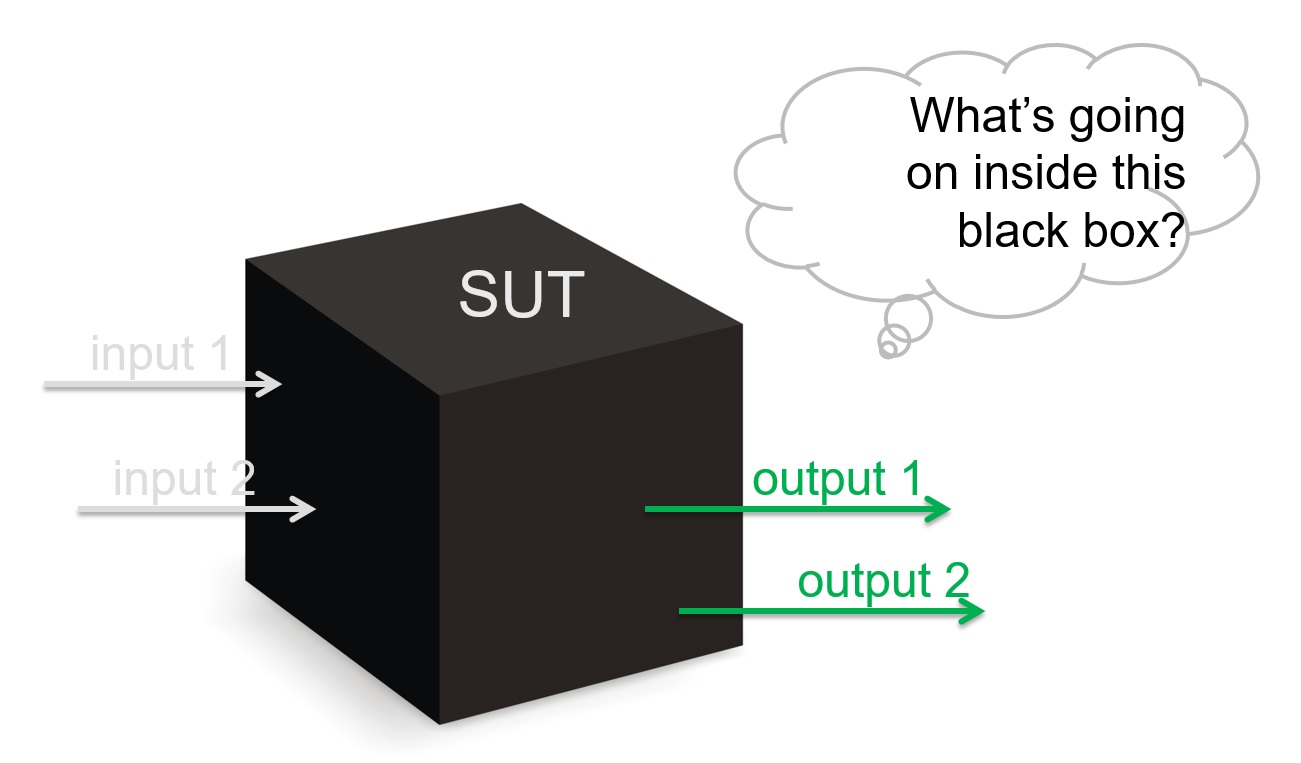
\includegraphics[width=.8\textwidth]{blackbox.jpg}
\end{center}


}



\frame{
	\frametitle{Our Research Method }
	
	\begin{center}
		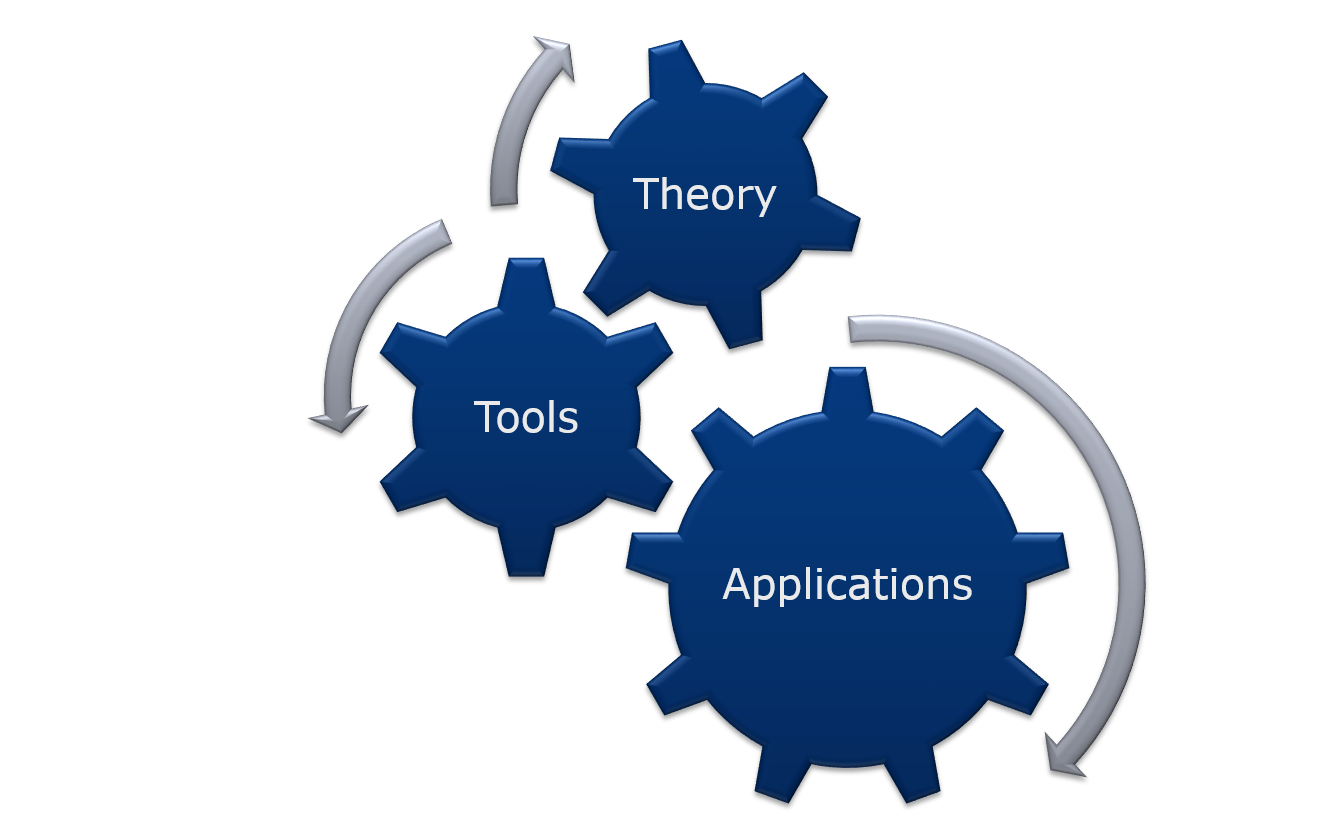
\includegraphics[width=.8\textwidth]{method.png}
	\end{center}
}



\frame{
	\frametitle{Bugs in Protocol Implementations}
	
	\begin{columns}
		\begin{column}{0.5\textwidth}  %%<--- here
			\begin{center}
				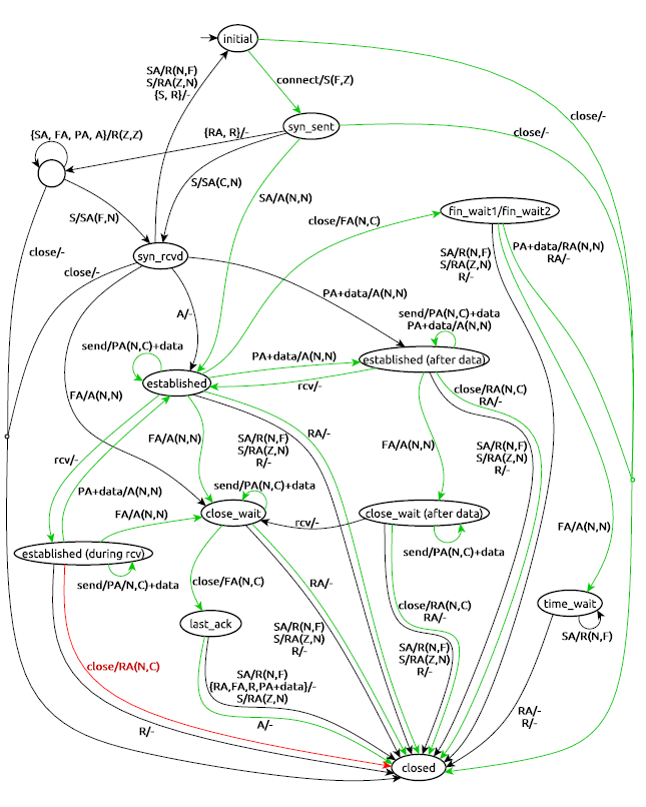
\includegraphics[width=0.9\textwidth]{TCPbug.png}
			\end{center}
		\end{column}
		\begin{column}{0.5\textwidth}
			Standard violations found in implementations of major protocols: 
			\begin{itemize}
				\item
				\blue{TLS}\  (Usenix Security'15)
				\item 
				\blue{TCP}\  (CAV'16)
				\item
				\blue{SSH}\  (Spin'17)
			\end{itemize}
			%
			\pause
			\red{These findings led to bug fixes in implementations.}
		\end{column}
	\end{columns}
	
}

\frame{
	\frametitle{ASML Challenge}
	
	\begin{columns}
		\begin{column}{0.5\textwidth}  %%<--- here
			\begin{center}
				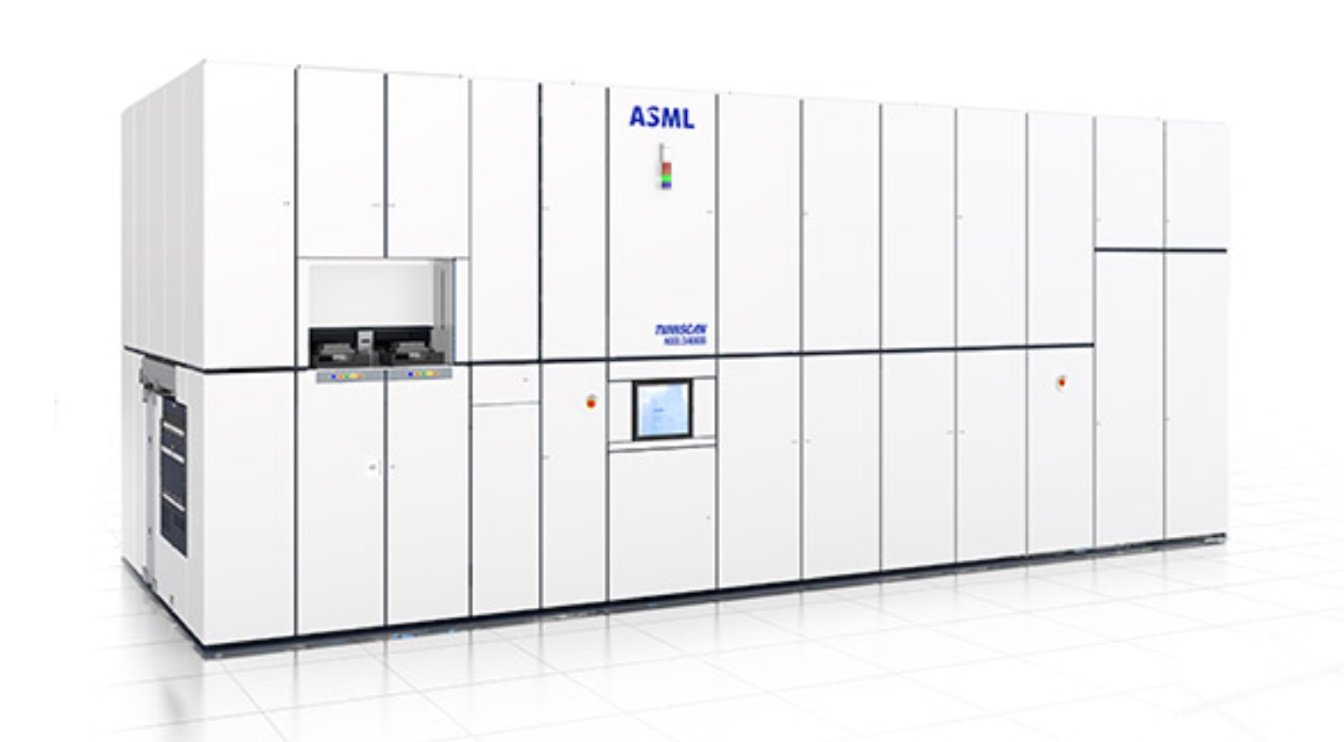
\includegraphics[width=0.9\textwidth]{ASML-Feature.jpg}
			\end{center}
		\end{column}
		\begin{column}{0.5\textwidth}
			Can active automata learning be used to support refactoring of legacy software at ASML?
			
			\vspace{1 em}
			ASML machines run on legacy software. Recent components have been designed using model-based techniques. Can we learn those?
			
			\vspace{1 em}
			Can we learn the hundreds of design and interface models
			used for high level control of the wafer flow during lot operation?
		\end{column}
	\end{columns}
	
}

\frame{
	\frametitle{Results LearnLib on ASML Benchmarks}
	
	\begin{center}
		\includegraphics[width=0.8\textwidth]{ASMLBenchmarks.jpg}
	\end{center}
	
}


\frame{
	\frametitle{Potential Applications Interface Models}
	
	\begin{center}
		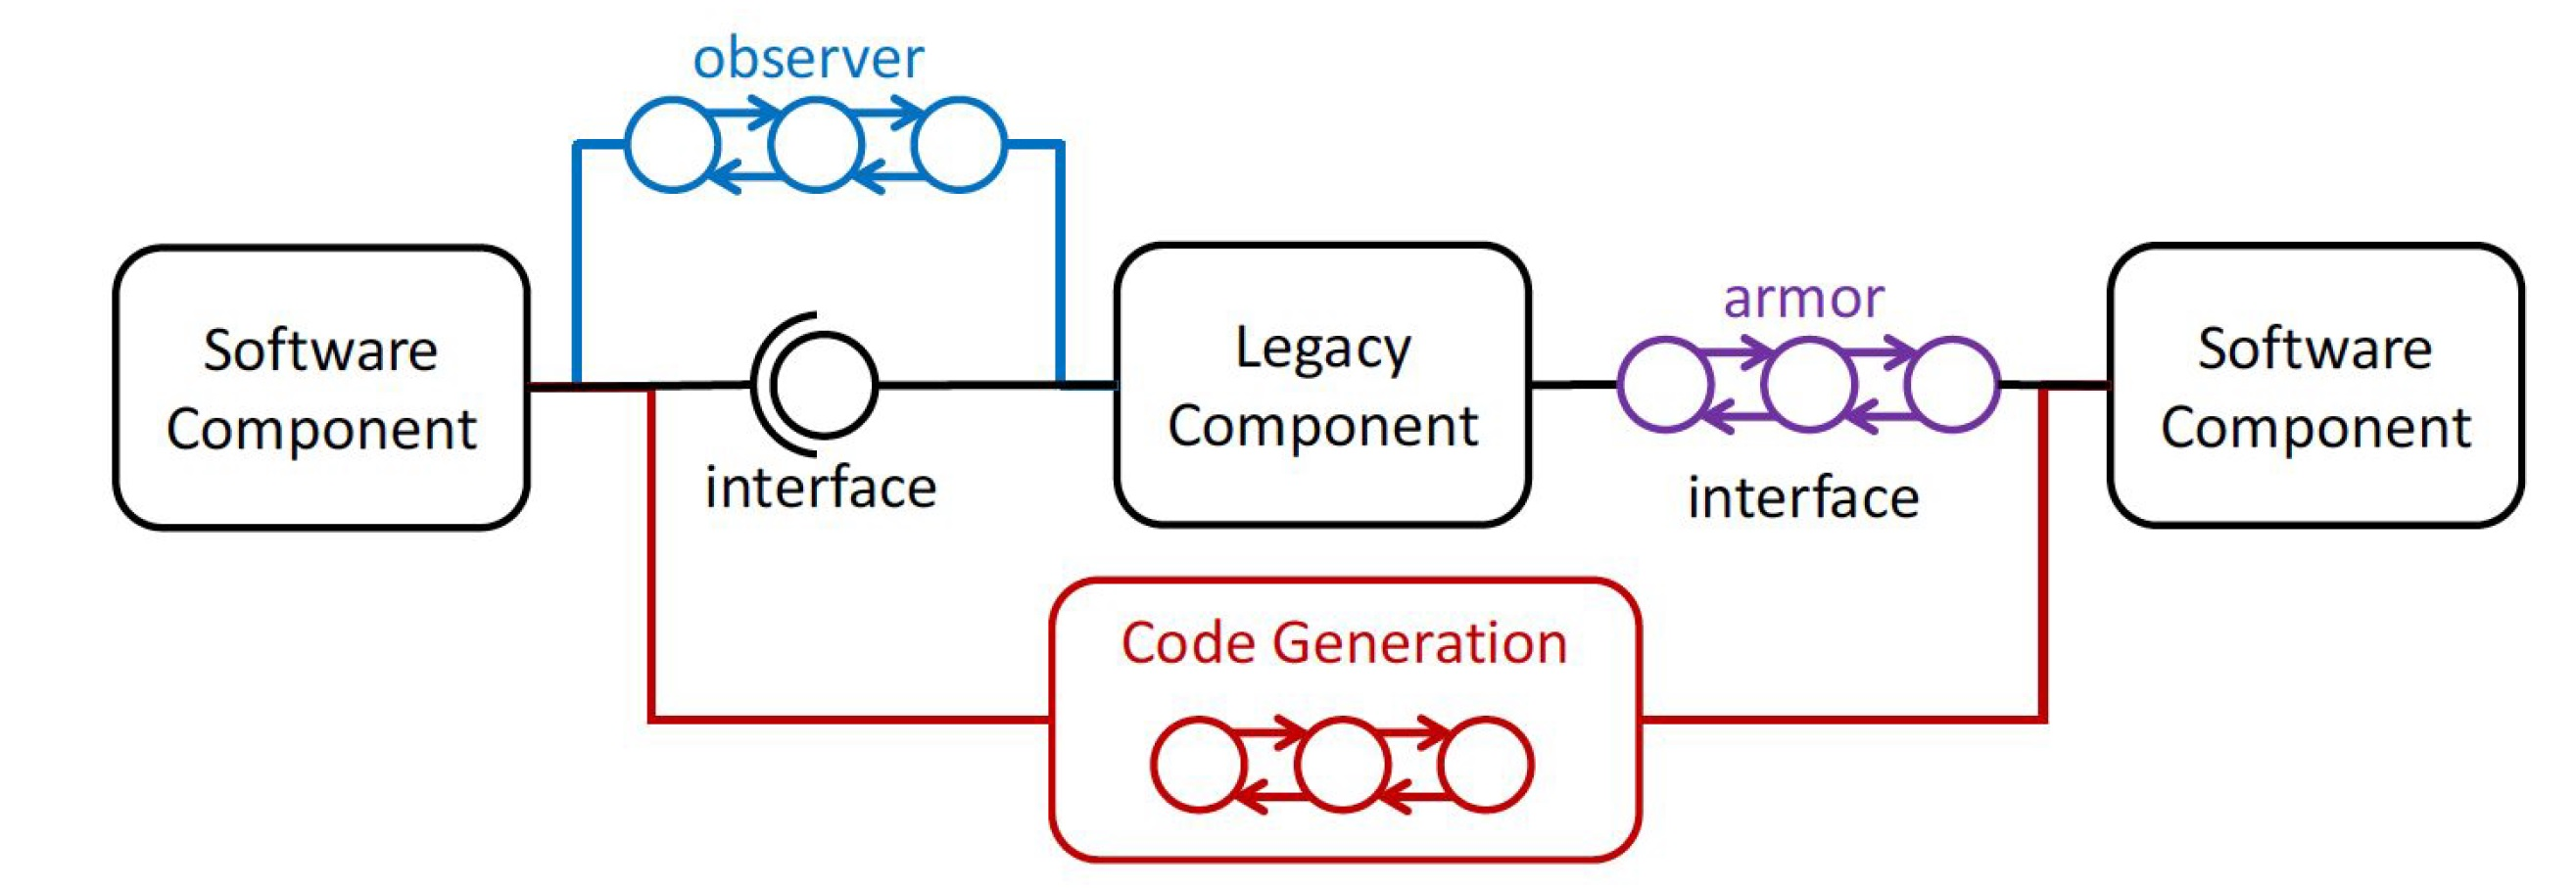
\includegraphics[width=\textwidth]{applicationsinterfacemodels}
	\end{center}
}





\frame{
	\frametitle{Future Work}
	\begin{enumerate}
		\item
		Learning EFSMs
		\item
		Combinations of black-box and white-box learning
		\item
		Improved algorithms for learning/testing
		\item
		From Mealy machines to I/O automata
		\item
		Adding time and probabilities
		\item
		Refactoring of legacy software excellent application domain
		\item
		Funding: NWO, TTW (via ESI), ERC,..
	\end{enumerate}
}







\end{document}
